\documentclass[aspectratio=169,11pt]{beamer}
\usepackage[T1]{fontenc}
\usepackage{lmodern,amsmath,amssymb,mathtools,bm,booktabs,array,graphicx,tikz}
\usetikzlibrary{arrows.meta,positioning,calc,decorations.pathreplacing,patterns}
\definecolor{ink}{HTML}{17344D}\definecolor{accent}{HTML}{087E8B}\definecolor{pale}{HTML}{EDF5F5}\definecolor{gold}{HTML}{AD6B19}
\providecommand{\dd}{\,\mathrm{d}}\providecommand{\R}{\mathbb{R}}
\providecommand{\E}{\mathbb{E}}\providecommand{\Var}{\operatorname{Var}}
\providecommand{\Cov}{\operatorname{Cov}}\providecommand{\diag}{\operatorname{diag}}
\providecommand{\norm}[1]{\left\lVert#1\right\rVert}
\providecommand{\abs}[1]{\left|#1\right|}
\usefonttheme{professionalfonts}
\setbeamercolor{normal text}{fg=black,bg=white}
\setbeamercolor{frametitle}{fg=ink,bg=white}
\setbeamercolor{title}{fg=ink}\setbeamercolor{structure}{fg=accent}
\setbeamercolor{block title}{fg=ink,bg=pale}\setbeamercolor{block body}{fg=black,bg=pale!40}
\setbeamercolor{alerted text}{fg=accent}
\setbeamerfont{frametitle}{size=\Large,series=\bfseries}
\setbeamerfont{title}{size=\LARGE,series=\bfseries}
\setbeamertemplate{navigation symbols}{}
\setbeamersize{text margin left=.7cm,text margin right=.7cm}
\setbeamertemplate{frametitle}{\vspace{.18cm}\insertframetitle\par\vspace{.1cm}{\color{accent}\hrule height .6pt}\vspace{.12cm}}
\newcommand{\notestarget}{notes.pdf}\newcommand{\noteslabel}{Notes}
\setbeamertemplate{footline}{\hspace{.7cm}\color{ink}\scriptsize Computational Cardiology\quad\href{\notestarget}{\noteslabel}\hfill\insertframenumber\,/\,\inserttotalframenumber\hspace{.7cm}\vspace{.18cm}}
\setbeamercovered{invisible}
\hypersetup{pdfauthor={Zan Ahmad},pdftitle={A periodically forced circulation},pdfpagemode=UseNone}
\begin{document}
\begin{frame}[plain]\vfill
{\small\color{accent} Computational Cardiology \quad Lecture 2}\par\medskip
{\raggedright\hyphenpenalty=10000\exhyphenpenalty=10000\LARGE\bfseries\color{ink} A periodically forced circulation}\par\bigskip
Zan Ahmad\par\smallskip
{\small Fall 2024}\par\vfill\end{frame}
\renewcommand{\notestarget}{notes.pdf\#note-pressure-volume-coordinates-and-cardiac-phase}
\begin{frame}[t,fragile,label=slide-stored-volumes-as-state-variables]{Stored volumes as state variables}
\[x_i=V_i-V_{d,i}=C_i(\phi)P_i.\]\pause{}\[\dot x=Bq,\qquad P=D_C(\phi)^{-1}x.\] Pressure requires both stored volume and phase.
\end{frame}
\renewcommand{\notestarget}{notes.pdf\#note-the-six-region-initial-value-problem}
\begin{frame}[t,fragile,label=slide-a-closed-six-region-network]{A closed six-region network}
The regions are LV, systemic arteries, systemic veins, RV, pulmonary arteries and pulmonary veins.\pause{} Four ideal valves and two open vascular beds connect them; no external reservoir appears.
\end{frame}
\renewcommand{\notestarget}{notes.pdf\#note-pressure-volume-coordinates-and-cardiac-phase}
\begin{frame}[t,fragile,label=slide-prescribed-cardiac-phase]{Prescribed cardiac phase}
\[\phi(t_s)=\phi(0)+Ft_s/60,\qquad T_b=60/F.\]\pause{} At $F=80\ \mathrm{min}^{-1}$, $T_b=0.75$ s. Both ventricles use the same clock.
\end{frame}
\renewcommand{\notestarget}{notes.pdf\#note-pressure-volume-coordinates-and-cardiac-phase}
\begin{frame}[t,fragile,label=slide-the-hydraulic-time-increment]{The hydraulic time increment}
\[h=\frac{0.001875}{60}=3.125\times10^{-5}\ \mathrm{min}.\]\pause{}\[Fh=\frac1{400}\ \text{cycle}.\] Flow in L/min must be multiplied by a step in minutes.
\end{frame}
\renewcommand{\notestarget}{notes.pdf\#note-pressure-volume-coordinates-and-cardiac-phase}
\begin{frame}[t,fragile,label=slide-the-initial-conserved-volume]{The initial conserved volume}
\[V_{\rm tot}(0)=\sum_i[V_{d,i}+C_i(0)P_i(0)]=5.13616\ \mathrm L.\]\pause{} Ventricular compliances at phase zero are $0.0146$ and $0.0365\ \mathrm{L/mmHg}$.
\end{frame}
\renewcommand{\notestarget}{notes.pdf\#note-periodic-forcing-and-the-return-map}
\begin{frame}[label=slide-a-periodically-forced-state-panel-1]{Pressure (mmHg)}
\centering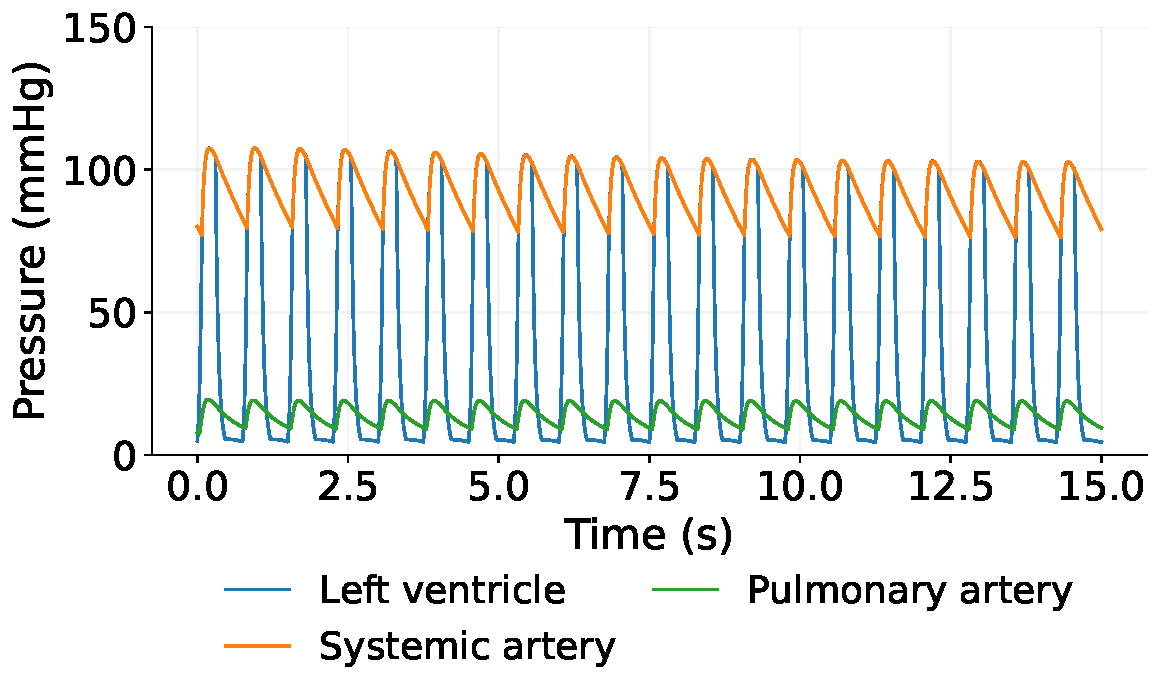
\includegraphics[width=.98\linewidth,height=.69\textheight,keepaspectratio]{presentation-figures/baseline-state-panel-1.pdf}\end{frame}
\renewcommand{\notestarget}{notes.pdf\#note-periodic-forcing-and-the-return-map}
\begin{frame}[label=slide-a-periodically-forced-state-panel-2]{Ventricular volume (mL)}
\centering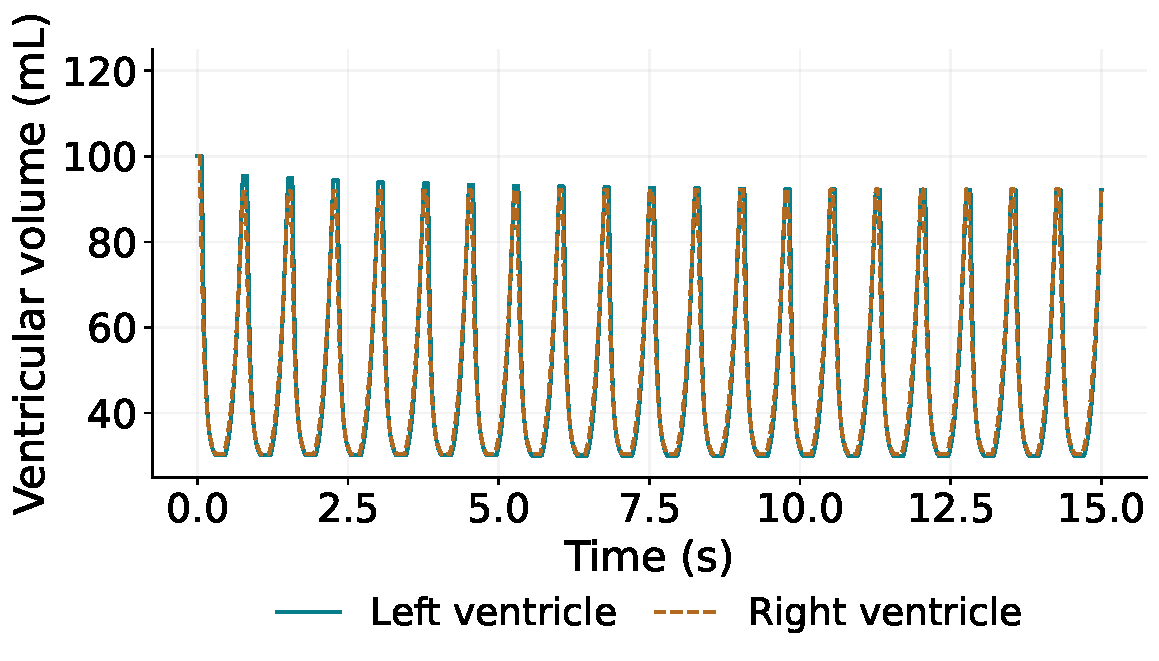
\includegraphics[width=.98\linewidth,height=.69\textheight,keepaspectratio]{presentation-figures/baseline-state-panel-2.pdf}\end{frame}
\renewcommand{\notestarget}{notes.pdf\#note-periodic-forcing-and-the-return-map}
\begin{frame}[t,fragile,label=slide-a-periodically-forced-state]{A periodically forced state}
Pressures and compartment volumes change throughout a beat. Total volume remains constant.\pause{}\[P(t+T_b)\simeq P(t)\] describes periodicity, not a stationary pressure.
\end{frame}
\renewcommand{\notestarget}{notes.pdf\#note-periodic-forcing-and-the-return-map}
\begin{frame}[t,fragile,label=slide-the-one-beat-return-map]{The one-beat return map}
\[x_{k+1}=\mathcal P(x_k),\qquad x_* =\mathcal P(x_*).\]\pause{} All comparisons use the same starting phase and initialized total volume.
\end{frame}
\renewcommand{\notestarget}{notes.pdf\#note-transient-decay-and-discretization-error}
\begin{frame}[t,fragile,label=slide-phase-aligned-comparison]{Phase-aligned comparison}
\[r_{\rm per}(t)=\max_i|P_i(t+T_b)-P_i(t)|.\]\pause{} A small return-map residual measures the remaining transient. It does not measure time-step error.
\end{frame}
\renewcommand{\notestarget}{notes.pdf\#note-the-discrete-volume-invariant}
\begin{frame}[t,fragile,label=slide-sum-the-compartment-equations]{Sum the compartment equations}
\[\dot V_i=(Bq)_i.\]\pause{}\[\frac{\mathrm d}{\mathrm dt}\sum_iV_i=\boldsymbol1^{\mathsf T}Bq=0.\] Every internal transfer occurs once with each sign.
\end{frame}
\renewcommand{\notestarget}{notes.pdf\#note-the-discrete-volume-invariant}
\begin{frame}[t,fragile,label=slide-the-same-invariant-after-a-time-step]{The same invariant after a time step}
\[D_C^{n+1}P^{n+1}-D_C^nP^n=hBq^{n+1}.\]\pause{} Left multiplication by $\boldsymbol1^{\mathsf T}$ removes every internal flow.
\end{frame}
\renewcommand{\notestarget}{notes.pdf\#note-the-discrete-volume-invariant}
\begin{frame}[label=slide-reconstruct-volume-at-the-saved-phase-panel-1]{Total blood volume (L)}
\centering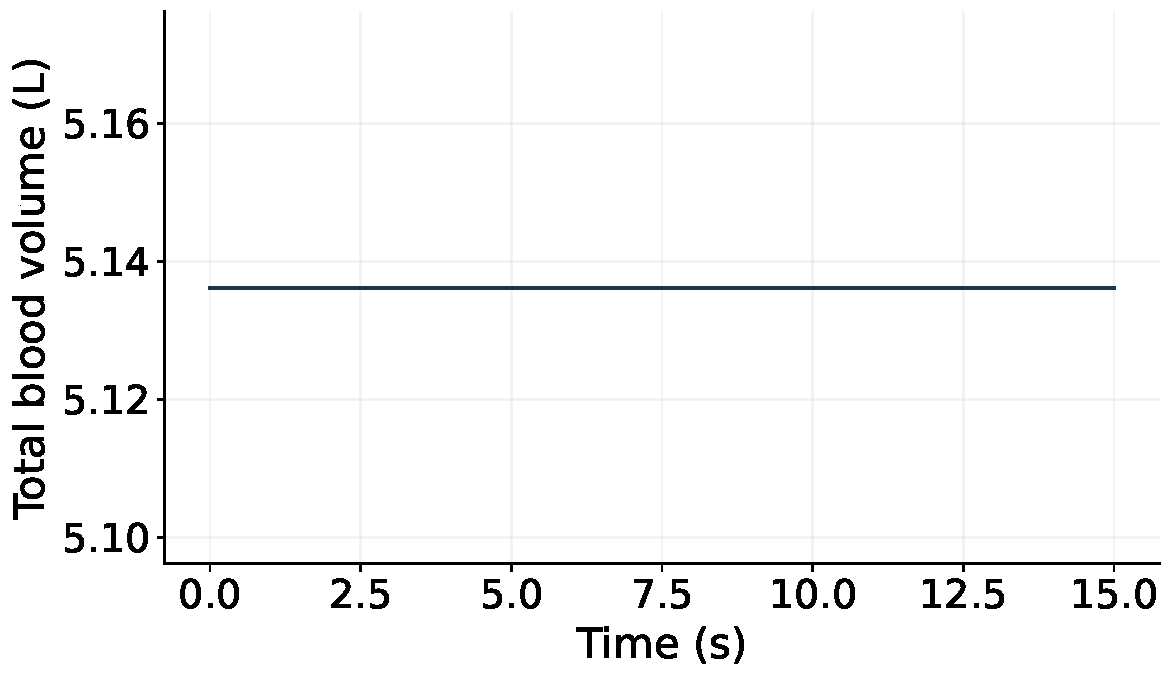
\includegraphics[width=.98\linewidth,height=.69\textheight,keepaspectratio]{presentation-figures/volume-audit-panel-1.pdf}\end{frame}
\renewcommand{\notestarget}{notes.pdf\#note-the-discrete-volume-invariant}
\begin{frame}[label=slide-reconstruct-volume-at-the-saved-phase-panel-2]{Total-volume drift (nL)}
\centering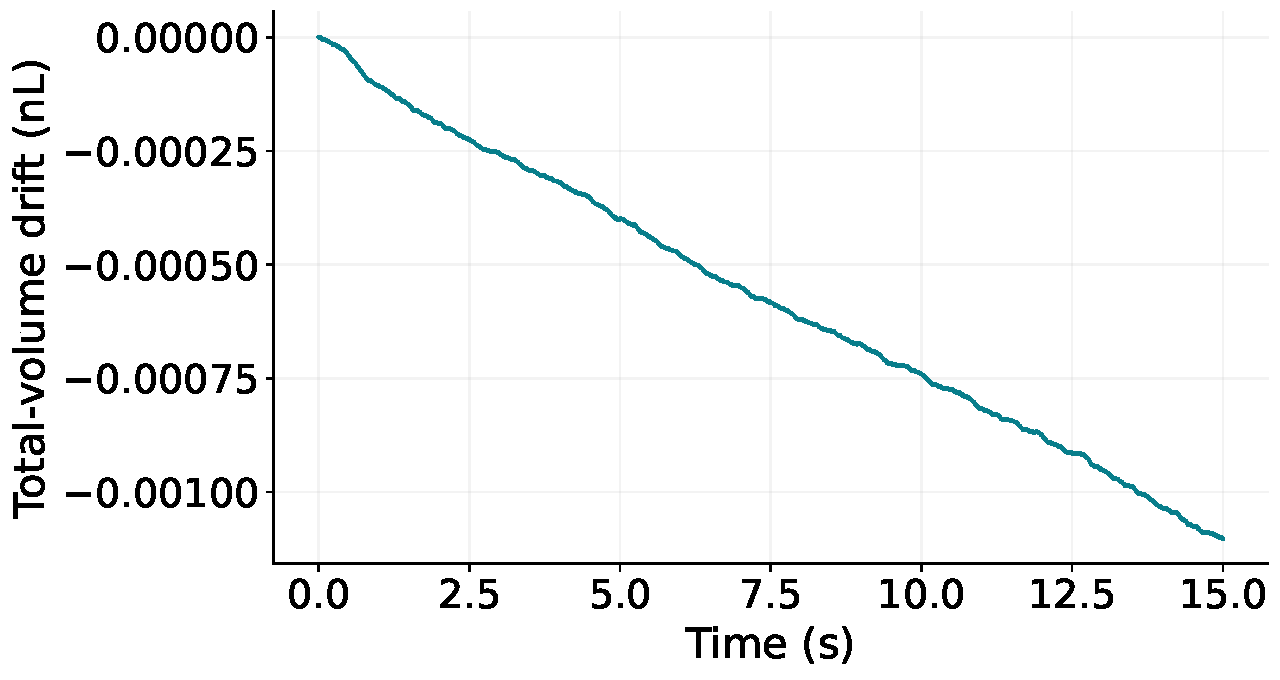
\includegraphics[width=.98\linewidth,height=.69\textheight,keepaspectratio]{presentation-figures/volume-audit-panel-2.pdf}\end{frame}
\renewcommand{\notestarget}{notes.pdf\#note-the-discrete-volume-invariant}
\begin{frame}[t,fragile,label=slide-reconstruct-volume-at-the-saved-phase]{Reconstruct volume at the saved phase}
\[\varepsilon_V(t)=\sum_i[V_{d,i}+C_i(\phi(t))P_i(t)]-V_{\rm tot}(0).\]\pause{} A fixed phase-zero compliance would measure a different quantity.
\end{frame}
\renewcommand{\notestarget}{notes.pdf\#note-the-discrete-volume-invariant}
\begin{frame}[t,fragile,label=slide-the-error-in-a-mismatched-diagnostic]{The error in a mismatched diagnostic}
\[V_{\rm wrong}(t)-V_{\rm true}(t)=\sum_i[C_i(0)-C_i(t)]P_i(t).\]\pause{} This term can be large without any loss of blood from the closed model.
\end{frame}
\renewcommand{\notestarget}{notes.pdf\#note-transient-decay-and-discretization-error}
\begin{frame}[t,fragile,label=slide-three-distinct-residuals]{Three distinct residuals}
\begin{align*}r_{\rm per}&=\|P_h(t+T_b)-P_h(t)\|_\infty,\\r_V&=|V_{{\rm tot},h}(t)-V_{\rm tot}(0)|,\\d_h&=\|P_h(t)-P_{h/2}(t)\|_\infty.\end{align*}\pause{} They measure periodicity, conservation and refinement sensitivity.
\end{frame}
\renewcommand{\notestarget}{notes.pdf\#note-constitutive-consistency-and-parameter-dependence}
\begin{frame}[t,fragile,label=slide-resistance-changes-the-dynamics]{Resistance changes the dynamics}
\[q_s=\frac{P_{sa}-P_{sv}}{R_s}.\]\pause{} Changing $R_s$ changes redistribution while leaving $\boldsymbol1^{\mathsf T}B=0$. Conservation does not require identical trajectories.
\end{frame}
\renewcommand{\notestarget}{notes.pdf\#note-constitutive-consistency-and-parameter-dependence}
\begin{frame}[t,fragile,label=slide-implicit-coupling]{Implicit coupling}
New compliances and new pressures enter the hydraulic balance together.\pause{} The pressure solve must also satisfy the ideal-valve inequalities; an algebraically conserved state can still have inconsistent valve labels.
\end{frame}
\end{document}
